\begin{figure}[t]
  \hspace{0.05\textwidth}%
  \begin{subfigure}[b]{\textwidth}
    \tikzstyle{legend-point}=[circle, inner sep=2pt]
    \definecolor{GraphBlue}{HTML}{6c8abd}
    \definecolor{GraphGreen}{HTML}{73b584}
    \definecolor{GraphRed}{HTML}{d07175}
    
    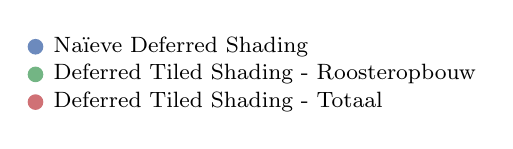
\begin{tikzpicture}
      \node (legend:naive) at (0.1\textwidth,  0pt)
            [legend-point, fill={GraphBlue}, label=right:{\footnotesize Na\"ieve Deferred Shading}] {};
      \node (legend:grid) at (0.1\textwidth, -10pt)
            [legend-point, fill={GraphGreen}, label=right:{\footnotesize Deferred Tiled Shading - Roosteropbouw}] {};
      \node (legend:tiled) at (0.1\textwidth, -20pt)
            [legend-point, fill={GraphRed}, label=right:{\footnotesize Deferred Tiled Shading - Totaal}] {};
    \end{tikzpicture}
  \end{subfigure}\hfill\\
  \begin{adjustbox}{minipage=\textwidth, scale=0.55}
    \begin{subfigure}[b]{0.8\textwidth}
      \centering
      \def\svgwidth{\textwidth}
      \input{./img/raw/ts-frames/deferred/frames_spaceship-indoor_70_320_32.pdf_tex}
      \caption{Spaceship indoor: $70$ lichten, $320^2$ pixels.}
      \label{fig:ts-frames-deferred:indoor-low}
    \end{subfigure}
  \end{adjustbox}\hspace{-0.075\textwidth}  %
  %
  \begin{adjustbox}{minipage=\textwidth, scale=0.55}
    \begin{subfigure}[b]{0.8\textwidth}
      \centering
      \def\svgwidth{\textwidth}
      \input{./img/raw/ts-frames/deferred/frames_spaceship-indoor_1260_2560_32.pdf_tex}
      \caption{Spaceship indoor: $1260$ lichten, $2560^2$ pixels.}
      \label{fig:ts-frames-deferred:indoor-high}
    \end{subfigure}
  \end{adjustbox} \\
  %
  \begin{adjustbox}{minipage=\textwidth, scale=0.55}
    \begin{subfigure}[b]{0.8\textwidth}
      \centering
      \def\svgwidth{\textwidth}
      \input{./img/raw/ts-frames/deferred/frames_pipers-alley_58_320_32.pdf_tex}
      \caption{Pipers Alley: $58$ lichten, $320^2$ pixels.}
      \label{fig:ts-frames-deferred:alley-low}
    \end{subfigure}
  \end{adjustbox}\hspace{-0.075\textwidth}  %
  %
  \begin{adjustbox}{minipage=\textwidth, scale=0.55}
    \begin{subfigure}[b]{0.8\textwidth}
      \centering
      \def\svgwidth{\textwidth}
      \input{./img/raw/ts-frames/deferred/frames_pipers-alley_1044_2560_32.pdf_tex}
      \caption{Pipers Alley: $1044$ lichten, $2560^2$ pixels.}
      \label{fig:ts-frames-deferred:alley-high}
    \end{subfigure}
  \end{adjustbox} \\
  %
  \begin{adjustbox}{minipage=\textwidth, scale=0.55}
    \begin{subfigure}[b]{0.8\textwidth}
      \centering
      \def\svgwidth{\textwidth}
      \input{./img/raw/ts-frames/deferred/frames_ziggurat-city_65_320_32.pdf_tex}
      \caption{Ziggurat stad: $65$ lichten, $320^2$ pixels.}
      \label{fig:ts-frames-deferred:city-low}
    \end{subfigure}
  \end{adjustbox}\hspace{-0.075\textwidth}  %
  %
  \begin{adjustbox}{minipage=\textwidth, scale=0.55}
    \begin{subfigure}[b]{0.8\textwidth}
      \centering
      \def\svgwidth{\textwidth}
      \input{./img/raw/ts-frames/deferred/frames_ziggurat-city_1170_2560_32.pdf_tex}
      \caption{Ziggurat stad: $1170$ lichten, $2560$ pixels.}
      \label{fig:ts-frames-deferred:city-high}
    \end{subfigure}
  \end{adjustbox}
  \caption{Overzicht van de uitvoeringstijd voor deferred shading per frame voor de
           drie testscenes bij verschillende resolutie en groottes van aantal
           lichten.}
  \label{fig:ts-frames-deferred}
\end{figure}

